% Two recurring problems of metaheuristics. Adapted from the CAEPIA 2026 slides.
\documentclass[border=0pt]{standalone}
% Shared preamble of the GSO-RL documentation figures.
% Compiled with latex (DVI) + dvisvgm; see ../build.sh.
\def\pgfsysdriver{pgfsys-dvisvgm.def}
\usepackage[T1]{fontenc}
\usepackage{lmodern}
\renewcommand{\familydefault}{\sfdefault}
\usepackage{amsmath, amssymb}
\usepackage{tikz}
\usetikzlibrary{positioning, shapes, arrows.meta, calc, fit, backgrounds}

% Palette
\definecolor{Purple}{RGB}{102, 0, 153}
\colorlet{ColMa}{green!50!black}   % macro-move M1
\colorlet{ColMb}{blue!70!black}    % macro-move M2
\colorlet{ColMc}{orange!85!black}  % macro-move M3
\definecolor{cGa}{RGB}{38, 166, 154}
\definecolor{cGb}{RGB}{229, 96, 76}
\definecolor{cGc}{RGB}{235, 165, 40}
\definecolor{cGd}{RGB}{125, 125, 215}
\definecolor{cGe}{RGB}{190, 60, 150}

% White background so figures stay readable in dark mode. The white rectangle lives on the
% "background" layer; figures draw their own backdrops on "behind", which sits above it.
\pgfdeclarelayer{behind}
\pgfsetlayers{background,behind,main}
\tikzset{every picture/.append style={show background rectangle,
  background rectangle/.style={fill=white, draw=none}, inner frame sep=8pt}}
% NOTE: with dvisvgm, text placed after a \color{...} group inside the same node is misplaced.
% Put differently coloured pieces of text in separate nodes.

\newcommand{\yes}{{\color{green!50!black}\checkmark}}
\newcommand{\nope}{{\color{red!70!black}$\boldsymbol{\times}$}}

% A region: guide with three concentric rings.  \guia[style]{x}{y}{color}{label}
\newcommand{\guia}[5][]{%
  \fill[#4!10, #1] (#2,#3) circle (1.05);
  \fill[#4!20, #1] (#2,#3) circle (0.7);
  \fill[#4!35, #1] (#2,#3) circle (0.35);
  \foreach \r in {0.35,0.7,1.05} \draw[#4, #1] (#2,#3) circle (\r);
  \fill[#4!80!black, #1] (#2,#3) circle (2pt);
  \node[#4!75!black, font=\scriptsize\bfseries, #1] at (#2,#3+1.22) {#5};
}

\begin{document}
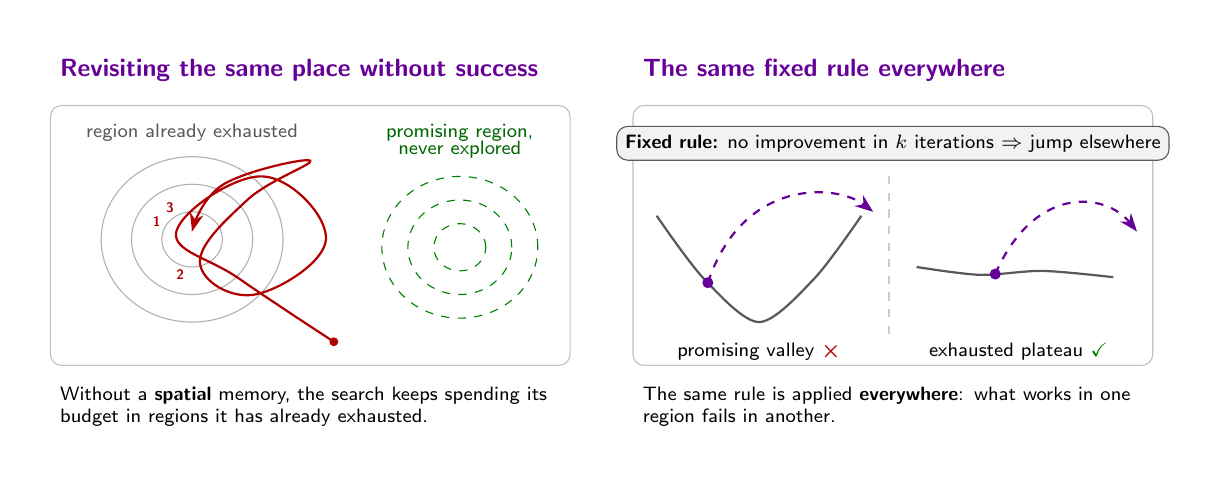
\begin{tikzpicture}[>=Stealth]
  % ---- Left: revisiting the same place ----
  \begin{scope}
    \node[anchor=west, font=\small\bfseries, Purple] at (-0.2,3.55) {Revisiting the same place without success};
    \draw[gray!50, rounded corners] (-0.2,-0.2) rectangle (6.4,3.1);
    \foreach \r in {0.35,0.7,1.05} \draw[gray!60] (1.6,1.4) ellipse ({\r*1.1} and \r);
    \node[font=\scriptsize, gray!70!black] at (1.6,2.75) {region already exhausted};
    \foreach \r in {0.3,0.6,0.9} \draw[green!50!black, dashed] (5,1.3) ellipse ({\r*1.1} and \r);
    \node[font=\scriptsize, green!40!black, align=center] at (5,2.65) {promising region,\\[-2pt] never explored};
    \draw[->, thick, red!70!black] plot[smooth, tension=0.7] coordinates {
      (3.4,0.1) (2.2,0.9) (1.4,1.5) (2.5,2.2) (3.3,1.4) (2.4,0.7) (1.7,1.1)
      (2.3,1.9) (3.1,2.4) (2.0,2.1) (1.6,1.5)};
    \fill[red!70!black] (3.4,0.1) circle (1.6pt);
    \node[font=\tiny\bfseries, red!70!black] at (1.15,1.62) {1};
    \node[font=\tiny\bfseries, red!70!black] at (1.45,0.95) {2};
    \node[font=\tiny\bfseries, red!70!black] at (1.32,1.8) {3};
    \node[anchor=north west, font=\scriptsize, text width=6.4cm] at (-0.2,-0.35)
      {Without a \textbf{spatial} memory, the search keeps spending its budget in regions it has already exhausted.};
  \end{scope}
  % ---- Right: the same fixed rule everywhere ----
  \begin{scope}[shift={(7.4,0)}]
    \node[anchor=west, font=\small\bfseries, Purple] at (-0.2,3.55) {The same fixed rule everywhere};
    \draw[gray!50, rounded corners] (-0.2,-0.2) rectangle (6.4,3.1);
    \node[draw=gray!70!black, fill=gray!10, rounded corners, font=\scriptsize, align=center, inner sep=3pt] at (3.1,2.62)
      {\textbf{Fixed rule:} no improvement in $k$ iterations $\Rightarrow$ jump elsewhere};
    \draw[thick, gray!70!black] plot[smooth] coordinates {(0.1,1.7) (0.7,0.9) (1.4,0.35) (2.1,0.9) (2.7,1.7)};
    \fill[Purple] (0.75,0.85) circle (2pt);
    \draw[->, thick, Purple, dashed] (0.75,0.85) .. controls (1.2,2.2) and (2.4,2.1) .. (2.85,1.75);
    \node[font=\scriptsize] at (1.4,-0.02) {promising valley \nope};
    \draw[thick, gray!70!black] plot[smooth] coordinates {(3.4,1.05) (4.2,0.95) (5,1.0) (5.9,0.92)};
    \fill[Purple] (4.4,0.96) circle (2pt);
    \draw[->, thick, Purple, dashed] (4.4,0.96) .. controls (4.9,2.1) and (5.8,2.0) .. (6.2,1.5);
    \node[font=\scriptsize] at (4.7,-0.02) {exhausted plateau \yes};
    \draw[gray!40, dashed] (3.05,0.2) -- (3.05,2.25);
    \node[anchor=north west, font=\scriptsize, text width=6.4cm] at (-0.2,-0.35)
      {The same rule is applied \textbf{everywhere}: what works in one region fails in another.};
  \end{scope}
\end{tikzpicture}
\end{document}
